\chapter{Procesamiento Lenguaje Natural}
\label{chap:pln}

\section{Introducción al Procesamiento del Lenguaje Natural}

El \acrfull{pln} es la rama de la \gls{ia} encargada de la interacción entre computadoras y el lenguaje humano. Este campo integra la lingüística computacional, basada en el modelado de reglas del lenguaje, con modelos estadísticos y algoritmos de aprendizaje profundo (\gls{dl}) y aprendizaje automático (\gls{ml}) \cite{stryker_what_nlp}.

El \gls{pln} forma parte a día de hoy de muchos motores de búsqueda, chatbots para atención al cliente (ya sea por escrito o por voz), y asistentes digitales como Alexa de Amazon o Siri de Apple.

El campo de la computación lingüística incluye tradicionalmente diversas fases para el análisis. Para el análisis de las palabras existen dos enfoques principales:

\begin{itemize}
      \item \textbf{Análisis de dependencias:} Examina las relaciones gramaticales binarias entre las palabras, identificando, por ejemplo, qué palabra modifica a cuál o cuál es el sujeto y el verbo principal.

      \item \textbf{Análisis de constituyentes:} Construye un árbol sintáctico que representa la estructura gramatical anidada de una oración, descomponiéndola en sintagmas o frases ordenadas jerárquicamente.
\end{itemize}

\section{Fases del \glsentryshort{pln}}

Las fases para realizar el \gls{pln} se pueden observar en la Figura \ref{fig:FasesNLP}:

\begin{figure}[h]
      \centering
      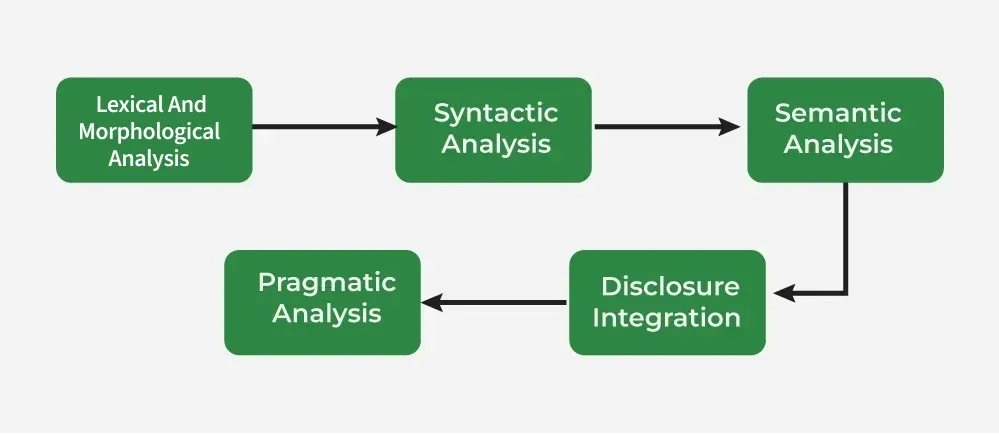
\includegraphics[width=1.0\linewidth]{imagenes/FasesNLP.png}
      \caption{Esquema de las fases del \gls{pln}. Extraído de \cite{geeksforgeeks_phases_nlp_2025}.}
      \label{fig:FasesNLP}
\end{figure}

A continuación, basándose en la estructura descrita en \cite{geeksforgeeks_phases_nlp_2025}, se detalla en qué consiste cada una de estas fases:

\subsection{Preprocesamiento y Tokenización}

Esta fase constituye el nivel inicial del procesamiento lingüístico computacional. Su propósito fundamental es transformar el texto crudo en una secuencia estructurada de unidades discretas y manejables. Para lograrlo, se integran diversas tareas de análisis léxico y morfológico que preparan la información para las etapas posteriores.

\begin{enumerate}
      \item \textbf{Preprocesamiento:} Esta fase inicial comprende un conjunto de operaciones destinadas a homogeneizar el texto. Entre las principales subtareas se encuentran la limpieza del contenido, la normalización (como la conversión a minúsculas) y la eliminación de caracteres especiales. Adicionalmente, suele llevarse a cabo la supresión de las \textit{stopwords}, que son palabras de muy alta frecuencia pero que carecen de una gran carga semántica (tales como ``el'', ``de'', ``y''). Como parte de este preprocesamiento, también se aplican técnicas de análisis morfológico para estandarizar el vocabulario:
            \begin{itemize}
                  \item \textit{Lematización:} Consiste en convertir las palabras a su forma base o lema canónico (por ejemplo, el verbo ``soy'' se transforma en ``ser'').
                  \item \textit{Stemming:} Se basa en reducir las palabras a su raíz léxica, eliminando sufijos y prefijos (por ejemplo, ``niñero'' se reduce a ``niño'').
            \end{itemize}

      \item \textbf{Tokenización:} Representa el proceso crítico mediante el cual se segmenta el flujo de texto en unidades atómicas significativas, denominadas \textit{tokens}.

            A modo de ejemplo, la oración \textit{Me gusta programar} se dividiría en la siguiente lista de tokens: \texttt{[``Me'', ``gusta'', ``programar'']}.

            La granularidad de los tokens depende del modelo empleado. Pueden corresponder a palabras completas, subpalabras (una técnica común en los modelos de tipo \gls{gpt}) o incluso a caracteres individuales. Una vez completada la tokenización, a cada token se le asigna un índice numérico único dentro de un vocabulario, un paso indispensable para la posterior generación de representaciones vectoriales o \textit{Embeddings} (concepto que se desarrollará en detalle en el Capítulo \ref{chap:word_embeddings}).

      \item \textbf{Etiquetado gramatical (\gls{pos} Tagging):} En esta etapa se asigna a cada token su correspondiente categoría morfológica (como sustantivo, verbo, adjetivo, entre otras), tomando en consideración tanto su definición formal como el contexto en el que aparece. Esto resulta esencial para desambiguar la función sintáctica que desempeña cada palabra en la oración.

            Siguiendo con el ejemplo anterior, el etiquetado de los tokens daría como resultado: \texttt{[``Me'' $\rightarrow$ Pronombre, ``gusta'' $\rightarrow$ Verbo, ``programar'' $\rightarrow$ Verbo]}.
\end{enumerate}

\subsection{Análisis sintáctico}

El análisis sintáctico examina la organización de las palabras dentro de una oración para verificar que se cumple con las reglas gramaticales del idioma. El objetivo fundamental de esta fase es la generación de un \textbf{árbol de análisis sintáctico}, el cual representa jerárquicamente la estructura gramatical del texto analizado. Esta representación estructurada permite a los sistemas computacionales interpretar las relaciones de dependencia y jerarquía entre los distintos elementos léxicos. Las tareas principales que abarca son:

\begin{itemize}
      \item \textbf{Etiquetado gramatical:} Se fundamenta en el proceso de \gls{pos} Tagging explicado en la fase de \textit{Preprocesamiento y Tokenización}. En esta etapa de análisis sintáctico, las categorías morfológicas previamente asignadas a cada token se utilizan para validar la corrección de la estructura jerárquica de la oración.
      \item \textbf{Resolución de ambigüedad sintáctica:} Consiste en determinar la estructura gramatical correcta cuando una oración puede analizarse de múltiples formas. Por ejemplo, en la frase \textit{Vi al hombre con el telescopio}, el sistema debe resolver si el telescopio es el instrumento utilizado por el sujeto para ver, o si es un objeto que lleva consigo el hombre.
\end{itemize}

\subsection{Análisis semántico}

Esta fase se centra en la coherencia lógica y la relevancia contextual del enunciado. Su objetivo principal es interpretar el significado de las palabras, analizando tanto su definición de diccionario como su variación según el contexto de uso. De este modo, se busca comprender el rol semántico de cada palabra para construir una representación lógica del mensaje. Las tareas fundamentales que abarca esta fase son:

\begin{enumerate}
      \item \textbf{\gls{ner}:} Se ocupa de la identificación y clasificación de elementos clave en el texto, tales como nombres de personas, ubicaciones geográficas, organizaciones, etc.
            \\
            Ejemplo: En la oración \textit{Mercedes anunció un nuevo coche en Berlín}, el sistema \gls{ner} identificaría a \textit{Mercedes} como una \textit{Organización} y a \textit{Berlín} como un \textit{Lugar}.

      \item \textbf{\gls{wsd}:} Consiste en identificar el significado exacto de una palabra polisémica basándose en el contexto en el que se encuentra (proceso conocido como resolución de ambigüedad léxico-semántica).
            \\
            Ejemplo: El término \textit{banco} se interpreta como una \textit{entidad financiera} en la frase \textit{Fui a sacar dinero al banco}, pero adquiere el significado de \textit{asiento} en la oración \textit{Me senté en el banco del parque}.
\end{enumerate}

\subsection{Integración del discurso}

Este proceso analiza cómo las oraciones individuales se conectan y relacionan entre sí para entender el contexto global. El objetivo de esta fase es garantizar que el significado del texto mantenga su coherencia lógica a través de los distintos párrafos y frases. Los aspectos fundamentales de esta fase son:

\begin{itemize}
      \item \textbf{Resolución de anáforas:} Consiste en identificar la conexión entre un pronombre y lo mencionado previamente en el texto.
            \\
            Ejemplo: En la secuencia \textit{Esther fue a comprar. Ella compró fruta}, el sistema debe vincular el pronombre \textit{Ella} con \textit{Esther}.

      \item \textbf{Referencias contextuales:} Aborda la interpretación de palabras o expresiones cuyo significado completo depende intrínsecamente de la información proporcionada en oraciones anteriores o posteriores.
            \\
            Ejemplo: La frase \textit{Fue un buen día} adquiere un significado concreto únicamente si se analiza dentro del contexto de la conversación.
\end{itemize}

\subsection{Análisis pragmático}

Esta fase final analiza más allá de la interpretación literal de las oraciones para inferir el significado real que se pretende transmitir. A diferencia del análisis semántico, que se ocupa del significado proposicional de las palabras, el análisis pragmático examina factores como el tono y el contexto. Las tareas principales de esta fase son:

\begin{itemize}
      \item \textbf{Detección de intenciones:} El sistema debe ver el propósito de la comunicación (si es una petición, una queja, una orden, etc.).
            \\
            Ejemplo: Ante la pregunta \textit{¿Tienes hora?}, el análisis pragmático entiende que la intención real del usuario es saber qué hora es, no una pregunta de sí o no.

      \item \textbf{Interpretación de lenguaje figurado:} Se encarga de identificar metáforas, ironías o frases hechas.
            \\
            Ejemplo: En la expresión \textit{Echar una mano}, el análisis pragmático entiende que significa \textit{ayudar a alguien}.
\end{itemize}

